% !TeX spellcheck = ca
\documentclass{article}
\usepackage[utf8]{inputenc}
\usepackage{amsmath}
\usepackage{ amssymb }
\usepackage{float}
\usepackage{graphicx}

%Tot això hauria d'anar en un pkg, però no sé com és fa
\newcommand*{\assignatura}[1]{\gdef\1assignatura{#1}}
\newcommand*{\grup}[1]{\gdef\3grup{#1}}
\newcommand*{\professorat}[1]{\gdef\4professorat{#1}}
\renewcommand{\title}[1]{\gdef\5title{#1}}
\renewcommand{\author}[1]{\gdef\6author{#1}}
\renewcommand{\date}[1]{\gdef\7date{#1}}
\renewcommand{\baselinestretch}{1.5}
\renewcommand{\maketitle}{ %fa el maketitle de nou
	\begin{titlepage}
		\raggedright{UNIVERSITAT DE LLEIDA \\
			Escola Politècnica Superior \\
			Grau en Enginyeria Informàtica\\
			\1assignatura\\}
		\vspace{5cm}
		\centering\huge{\5title \\}
		\vspace{3cm}
		\large{\6author} \\
		\normalsize{\3grup}
		\vfill
		Professorat : \4professorat \\
		Data : \7date
\end{titlepage}}
%Emplenar a partir d'aquí per a fer el títol : no se com es fa el package
%S'han de renombrar totes, inclús date, si un camp es deixa en blanc no apareix


\title{Práctica de Modelos Probabilísticos - Predicción de la valoración de alojamientos de AirBnB}
\author{Joaquim Picó Mora, Ian Palacín Aliana, Aiax Faura Vilalta}
\date{Dilluns 8 Juny}
\assignatura{Aprenentatge i Raonament Automàtic}
\professorat{R.Bejar}
\grup{}

\renewcommand{\refname}{Bibliografia}

%Comença el document
\begin{document}
	\maketitle
	\thispagestyle{empty}


\section{Generador d'arff}	
% Explicació de com executar l'script
L'script està realitzat amb python 3, així que una forma d'executar-lo és fent:
\begin{verbatim}
python3 generate_arff.py <data-set> <out-learning-dataset> <out-evaluation-dataset>
\end{verbatim}
També es pot executar directament donant permisos d'execució al fitxer python mitjançant:
\begin{verbatim}
chmod +x  generate_arff.py
./generate_arff.py <data-set> <out-learning-dataset> <out-evaluation-dataset>
\end{verbatim}
On $<data-set>$ és el nom del data set d'entrada, en el nostre cas barca.csv, i $<out-learning-dataset>$ i $<out-evaluation-dataset>$ són el nom dels fitxers de sortida traduits a arff per a l'aprenentatge i l'avaluació de la xarxa.\\
A l'executar l'script, si no es fica el nombre d'arguments que és demana s'imprimeix un missatge amb el mètode d'ús i es surt del programa. 
\section{Puntuació dels models}
% Puntuació log(UPSM) i error de classificació  de tots els models
% de tots els models
\subsection{Classe 1}
\begin{table}[H]
\begin{tabular}{ll}
\hline
Error classificació & log(UPSM)           \\
\hline
48.6863 \%          & -103784.93516475169 \\
48.6863 \%          & -103845.33539207192 \\
48.9079 \%          & -103702.10859464137 \\
48.8762 \%          & -103940.05807545574 \\
48.8762 \%          & -103865.53730402223 \\
48.6863 \%          & -103799.35937336765 \\
48.8762 \%          & -104599.69306872078 \\
48.8762 \%          & -103840.89609789594 \\
48.9079 \%          & -103833.55088340564 \\
48.8762 \%          & -103892.78517133751
\end{tabular}
\end{table}
\subsection{Classe 2}
\begin{table}[H]
\begin{tabular}{ll}
\hline
Error classificació & log(UPSM)           \\
\hline
50.1108 \%          & -127916.12156930043
\end{tabular}
\end{table}
\subsection{Classe 3}
\begin{table}[H]
\begin{tabular}{ll}
\hline
Error classificació & log(UPSM)           \\
\hline
48.528  \%          & -105938.04552255767 \\
48.5597 \%          & -105871.05201856224 \\
49.0028 \%          & -106280.47076199797 \\
48.9712 \%          & -105640.32391213975 \\
48.1798 \%          & -105671.92496621847 \\
47.9899 \%          & -105982.94208430553 \\
49.446  \%          & -105844.14592852714 \\
48.2431 \%          & -105889.99653741406 \\
48.4014 \%          & -106654.81244066187 \\
48.6863 \%          & -105914.39769708786
\end{tabular}
\end{table}
\section{Millor model}
\subsection{Classe 1}
En aquest cas el millor model és el primer que apareix a la taula amb un error de 48.6863 \%. Tot i que veiem que hi ha dos altres models que tenen el mateix percentatge d'error de classificació, el que resulta tenir el UPSM score més alt és el primer.
\begin{figure}[H]
  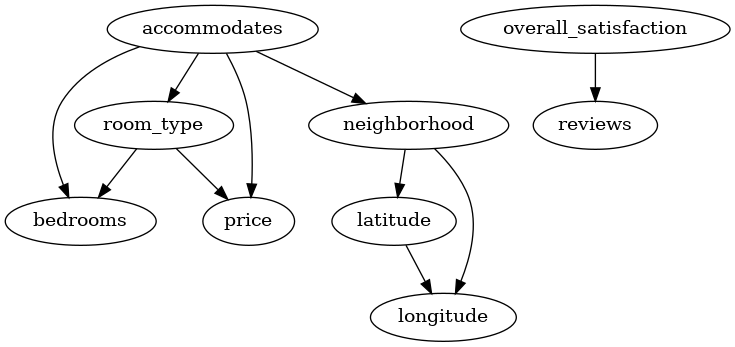
\includegraphics[width=\linewidth]{classe1.png}
  \caption{Graf dirigit xarxa classe 1.}
  \label{fig:gp1}
\end{figure}
\subsection{Classe 2}
Només hi pot haver un model ja que només hi ha una forma de generar la xarxa. El percentatge d'error és de 50.1108 \%.
\begin{figure}[H]
  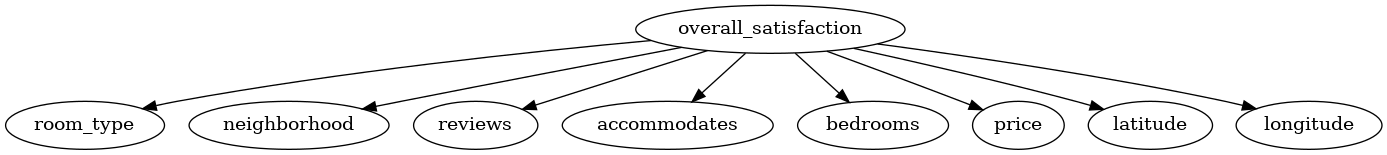
\includegraphics[width=\linewidth]{classe2.png}
  \caption{Graf dirigit xarxa classe 2.}
  \label{fig:gp2}
\end{figure}
\newpage
\subsection{Classe 3}
Aquí es veu mes clar que el millor model és el sisé que apareix a la taula, ja que és el que té el percentatge d'errors més baix amb valor 47.9899 \%.
\begin{figure}[H]
  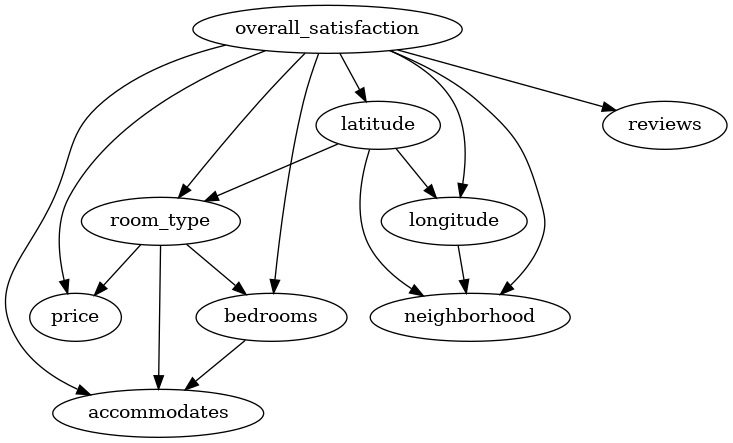
\includegraphics[width=\linewidth]{classe3.png}
  \caption{Graf dirigit xarxa classe 3.}
  \label{fig:gp3}
\end{figure}

\section{Mida dels dominis}
%Primer vam provar sense cap tipus de reducció
%Després vam probar a reduir latitut i longitud ja que era el camp que 
%tenia més valors diferents. Ho vam fer per quartils.
%Després també ens en vam adonar de que podiam reduir el preu i les reviews ja
%que eren camps quantitatius i per tant reductibles. Els vam "agrupar" de 20 en 20.
%Per overall satisfaction vam decidir canviar els simbols
%Podria ser que al haver tants valors diferents la xarxa entrenada acabes tenint
%molt overfeating.

%Importante: El que quiera obtener una nota superior al 8.5, deberá de explicar 
%con detalle de que forma
%ha escogido el tamaño de los conjuntos discretos de valores para transformar los
%atributos de entrada con
%valores reales. Y explicar si habéis probado con diferentes tamaños, y con que
%tamaños os habéis quedado
%finalmente (y el motivo).
\begin{itemize}
	\item \textbf{Latitud i longitud:} s'ha traduit el domini de la latitud i longitud 
	mitjançant quartils.
	Per calcular els valors que delimitaran els quartils, s'han ordenat tots els 
	valors segons la longitud i latitud, i s'han separat en 4 subsets. Totes les 
	coordenades que pertanyen al quartil 1 tindran el mateix valor, i el mateix
	passarà per la resta de quartils.
	D'aquesta manera es redueix l'àrea
	(de Barcelona en aquest cas) en una matriu 4x4. Això és una forma 
	representativa de reduir la latitud i longitud mantenint la coherència de la
	dada.

	\item \textbf{Overall satisfaction:} s'ha fet una traducció dels símbols, 
	passant-los a enters. En aquest cas no s'ha reduit el domini.

	\item \textbf{Price i review:} vist que el domini d'aquests atributs era molt 
	gran, també s'ha decidit fer una reducció. En aquest cas s'ha optat per 
	una divisió entera per tal de repartir-ho en rangs de 20.
\end{itemize}

Inicialment vam provar a utilitzar les dades sense cap tipus de reducció, el que
portava a milers de latituds i longituds. Fent-ho d'aquesta forma, el model 
d'entrenament a weka tardava massa, no vam arribar ni a veure els resultats.

El primer pas que vam fer va ser traduir solament latitud i longitud ja que era
l'atribut amb el domini més gran. Després d'entrenar el model al weka el 
percentatge d'error era aproximadament d'un 50\%.\\

Per veure si millorava l'entrenament, vam reduir també el preu i les reviews. El
percentatge d'error en aquest cas era gairebé idèntic al anterior, no obstant 
el temps d'entrenament era menor ja que el domini era més reduit, per tant 
ens vam quedat amb les reduccions.\\

Inicialment pensàvem que un 50\% d'errors era massa per un model amb aquest nombre 
de dades, però ens en vam adonar que la desviació de l'atribut overall\_satisfaction 
era molt poca. Per ser més específics, més de la meitat de les satisfaccions són 
de 4.5 (7504 de 12633).
Això ens porta a pensar que el que passa en el model és semblant a 
tirar una moneda per veure si la satisfacció serà 4.5 o no.  












\end{document}